\section{Preadmitere F aprilie 2024}

2024.P.1. Modulul variației energiei potențiale a unui corp ce coboară între două puncte ale unui plan înclinat este de 4 ori mai mare decât modulul lucrului mecanic al forței de frecare între aceleași puncte. Randamentul planului înclinat este: (9 pct.)\\ a) $0,8$; b) $0,4$; c) $0,6$; d) $0,2$; e) $0,5$; f) $0,3$.\\ Randamentul planului înclinat este:\\ $\eta=\frac{L_{u}}{L_{c}}=\frac{\Delta E_{p}}{\Delta E_{p}+L_{F f}}=\frac{4}{5}=0,8$. Răspuns corect a.\\

2024.P.2. O bilă este aruncată vertical în sus. Distanța dintre bilă și un punct fix de pe traiectoria acesteia este prezentată în figura de mai jos. Cunoscând $g=10 \mathrm{~m} / \mathrm{s}^{2}$, viteza cu care a fost aruncată bila este: (9 pct.)\\ a) $20 \mathrm{~m} / \mathrm{s}$; b) $8 \mathrm{~m} / \mathrm{s}$; c) $12 \mathrm{~m} / \mathrm{s}$; d) $4 \sqrt{10} \mathrm{~m} / \mathrm{s}$; e) $10 \sqrt{2} \mathrm{~m} / \mathrm{s}$; f) $4 \sqrt{15} \mathrm{~m} / \mathrm{s}$.\\ 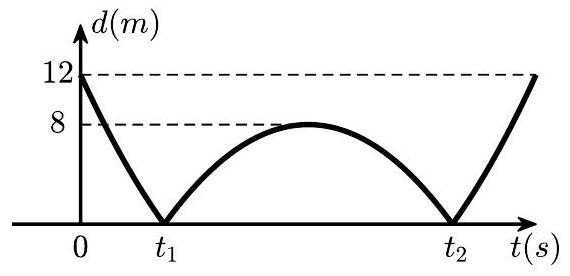
\includegraphics[width=0.4\linewidth]{images/2025_08_27_d74d983b3f0f59c27780g-1}\\ Aplicând legea lui Galilei, $v_{0}^{2}=2 a \Delta d \Rightarrow v_{0}=\sqrt{20 \cdot \Delta d}$, unde $v_{0}$ este viteza iniţială a bilei. Citind deplasarea din grafic, $\Delta d=8-(-12)=20 \mathrm{~m}$, obţinem $v_{0}=\sqrt{2 \cdot 10 \cdot 20} \Rightarrow v_{0}=20 \mathrm{~m} / \mathrm{s}$. Răspuns corect a.\\

2024.P.3. O gazelă vede o panteră aflată la o distanță $d=27 \mathrm{~m}$ și începe să alerge cu viteză constantă. În același moment, pantera pornește cu viteza inițială $v=32 \mathrm{~m} / \mathrm{s}$ în urmărirea gazelei. Mișcarea celor două animale se petrece pe dreapta determinată de pozițiile lor inițiale. Întrucât pantera nu poate alerga cu viteza maximă pe distanțe lungi, ea își reduce viteza brusc cu câte $3 \mathrm{~m} / \mathrm{s}$ la fiecare 2 secunde. Viteza minimă cu care trebuie să alerge gazela pentru a nu fi prinsă este: (9 pct.)\\ a) $24,5 \mathrm{~m} / \mathrm{s}$; b) $18,5 \mathrm{~m} / \mathrm{s}$; c) $23,75 \mathrm{~m} / \mathrm{s}$; d) $24,125 \mathrm{~m} / \mathrm{s}$; e) $27,5 \mathrm{~m} / \mathrm{s}$; f) $23,45 \mathrm{~m} / \mathrm{s}$.\\ Legile de mișcare ale celor două animale sunt: $x_{g}(N)=d_{0}+v_{g} N t_{0}\\ x_{p}(N)=v z_{0}+(v-\Delta v) t_{0}+\cdots{ }+(v-(N-1) \Delta v) t_{0}=N v t_{0}-\Delta v t_{0} N(N-1)$\\ Condițiile de întâlnire sunt:\\ $x_{g}=x_{p}$\\ $v_{g}<v-(N-1) \Delta v$\\ $v_{g}>v-N \Delta v$\\ Unde:\\ $v_{g}=\frac{x_{g}(N)-d_{0}}{N t_{n}}$\\ $v_{p}=v_{0}-\Delta v \frac{N(N-1)}{2}$\\ De aici rezultă: $N(N+1)<\frac{2 d_{0}}{\Delta v t_{n}}<N(N+1)$ şi se obține $N=3$.\\ Din condiţia $x_{g}=x_{p}$ rezultă $v_{g}=24,5 \mathrm{~m} / \mathrm{s}$. Răspuns corect a.\\

2024.P.4. Două vase $A$ și $B$ construite dintr-un material conductor termic sunt conectate între ele printr-un tub cu volum neglijabil confecționat din același material. Două robinete $C$ și $D$ sunt montate pe tuburi ca în figură. Inițial, vasele sunt vidate și robinetele închise. Se deschide robinetul $D$ și se umple vasul $B$ cu aer până când presiunea din vas este $p=1,2 \mathrm{~atm}$. Se închide robinetul $D$ și apoi se deschide robinetul $C$. Presiunea din vasul $B$ scade cu $\Delta p=0,2 \mathrm{~atm}$. Dacă volumul vasului $B$ este $V_{B}=10$ litri, volumul vasului $A$ este: (9 pct.)\\ a) 2 litri; b) 4 litri; c) 6 litri; d) 3 litri; e) 8 litri; f) 5 litri.\\ 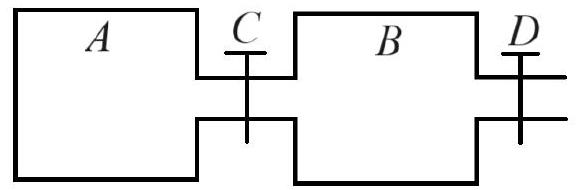
\includegraphics[width=0.4\linewidth]{images/2025_08_27_d74d983b3f0f59c27780g-2}\\ La momentul iniţial, gazul din vasul $B$ are $V_{B}=10 \mathrm{~l}$ şi $P i_{B}=1,2 \mathrm{~atm}$ iar vasul $A$ este vidat. Aplicăm ecuaţia termică de stare pentru gazul care intră în cele două vase in starea iniţială $P_{i} V_{B}=\nu R T$ şi în starea finală:\\ $P_{f}=(P_{i}-\Delta P) \cdot\left(V_{A}+V_{B}\right)=\nu R T$.\\ Din egalarea celor două ecuaţii se obţine $(P_{i}-\Delta P) \cdot\left(V_{A}+V_{B}\right)=P_{i} V_{B}$, de unde rezultă:\\ $\frac{V_{A}}{V_{R}}+1=\frac{P_{i}}{P_{i}-\Delta P}$ şi $\frac{V_{A}}{V_{R}}=\frac{P_{i}-P_{i}+\Delta P}{P_{i}-\Delta P} \Rightarrow V_{A}=V_{B} \cdot \frac{\Delta P}{P_{i}-\Delta P}=10 \cdot \frac{0,2}{1}=2 \mathrm{~l}$. Răspuns corect a.\\

2024.P.5. La funcționarea în gol a unei surse, tensiunea la borne este de $10 \mathrm{~V}$, iar la funcționarea în scurtcircuit curentul are intensitatea de $40 \mathrm{~A}$. Rezistența internă a sursei este: (9 pct.)\\ a) $0,25 \Omega$; b) $1 \Omega$; c) $2,5 \Omega$; d) $4 \Omega$; e) $0,4 \Omega$; f) $2 \Omega$.\\ La funcţionarea în gol a sursei, tensiunea electromotoare este egală cu tensiunea la bornele sursei $E=U_{G}$. În scurt circuit avem $I_{SC}=\frac{E}{r}=\frac{U_{G}}{r}$, de unde rezultă $r=0,25 \Omega$. Răspuns corect a.\\

2024.P.6. O coardă de alpinism având lungimea inițială de $60 \mathrm{~m}$ și aria secţiunii transversale egală cu $60 \mathrm{~mm}^{2}$ se alungește cu $1,5 \mathrm{~m}$ sub acțiunea greutății unui om cu masa de $90 \mathrm{~kg}$. Cunoscând $g=10 \mathrm{~m} / \mathrm{s}^{2}$, modulul lui Young pentru materialul din care este confecționată coarda este: (9 pct.)\\ a) $6 \cdot 10^{8} \frac{\mathrm{kg}}{\mathrm{m} \cdot \mathrm{~s}^{2}}$; b) $8 \cdot 10^{8} \frac{\mathrm{kg}}{\mathrm{m} \cdot \mathrm{~s}^{2}}$; c) $4 \cdot 10^{8} \frac{\mathrm{kg}}{\mathrm{m} \cdot \mathrm{~s}^{2}}$; d) $5 \cdot 10^{6} \frac{\mathrm{kg}}{\mathrm{m} \cdot \mathrm{~s}^{2}}$; e) $3,75 \cdot 10^{5} \frac{\mathrm{kg}}{\mathrm{m} \cdot \mathrm{~s}^{2}}$; f) $8 \cdot 10^{6} \frac{\mathrm{kg}}{\mathrm{m} \cdot \mathrm{~s}^{2}}$.\\ Modulul lui Young se determină din legea lui Hooke:\\ $E=\frac{\frac{F}{S}}{\frac{\Delta l}{l_{0}}}=6 \cdot 10^{-8} \mathrm{~N} / \mathrm{m}^{2}$. Răspuns corect a.\\

2024.P.7. Într-un vas închis cu volumul $V=1$ litru se află un gaz ideal monoatomic la presiunea $p_{i}=100 \mathrm{kPa}$. Gazul este încălzit izocor până la presiunea finală $p_{f}=120 \mathrm{kPa}$. Căldura absorbită de gaz este: (9 pct.)\\ a) $30 \mathrm{~J}$; b) $20 \mathrm{~J}$; c) $3 \mathrm{~kJ}$; d) $10 \mathrm{~kJ}$; e) $100 \mathrm{~kJ}$; f) $120 \mathrm{~J}$.\\ Temperatura finală a gazului se determină din legea transformării izocore:\\ $\frac{P_{1}}{T_{1}}=\frac{P_{2}}{T_{2}} \Rightarrow T_{2}=T_{1} \cdot \frac{P_{2}}{P_{1}}$.\\ Căldura absorbită este:\\ $Q=\nu \cdot C_{V} \cdot \Delta T=\frac{3}{2} \nu R \Delta T=\frac{3}{2} \nu R T_{1}\left(\frac{p_{2}}{p_{1}}-1\right)$, iar $T_{1}$ se determină din ecuaţia termică de stare $P_{1} V_{1}=\nu R T_{1} \Rightarrow T_{1} \frac{P_{1} V_{1}}{\nu R}$.\\ În final se obţine $Q=\frac{3}{2} P_{1} V_{1}\left(\frac{P_{2}}{P_{1}}-1\right)=\frac{3}{2} \cdot 10^{5} \mathrm{~Pa} \cdot 10^{-3} \cdot 0,2=30 \mathrm{~J}$. Răspuns corect a.\\

2024.P.8. Circuitul din figură este format dintr-un număr infinit de surse de tensiune, fiecare cu tensiunea electromotoare $E$ și rezistența internă $r=2 \Omega$, și un număr infinit de rezistoare, fiecare cu rezistența $4 r$. Știind că intensitatea curentului prin ampermetrul ideal este de $1 \mathrm{~A}$, tensiunea electromotoare $E$ este: (9 pct.)\\ a) $4(\sqrt{2}+1) V$; b) $2(\sqrt{2}+1) V$; c) $2(\sqrt{2}-1) V$; d) $2 \sqrt{2} V$; e) $4 \sqrt{2} V$; f) $2 \mathrm{~V}$.\\ 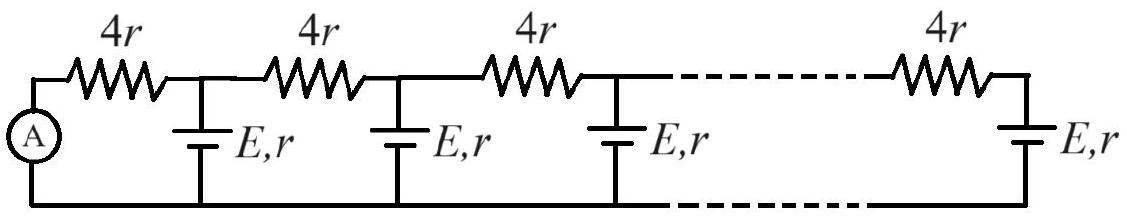
\includegraphics[width=0.4\linewidth]{images/2025_08_27_d74d983b3f0f59c27780g-3}\\ Rezistenţa echivalentă ($r_{e}$) a circuitului infinit este invariantă la adăugarea unei celule, deci putem scrie $\frac{1}{r_{R}}=\frac{1}{r}+\frac{1}{r_{R}+4 r}$, de aici rezultă ecuaţia:\\ $r_{e}^{2}+4 r_{e} r-4 r^{2}=0$ cu soluţia $r_{B}=2 r(\sqrt{2}+1)$;\\ Acelaşi lucru este valabil şi pentru tensiunea electromotoare echivalentă ($E_{e}$):\\ $E_{e}=\frac{\frac{E_{e}}{2 r(\sqrt{2}+1)}+\frac{E}{r}}{\frac{1}{r}+\frac{1}{2 r(\sqrt{2}+1)}}$, de unde se obţine $E_{e}=E$.\\ Aplicând legea lui Ohm, pe intregul circuit, avem:\\ $I=\frac{E}{2 r(\sqrt{2}+1)} \Rightarrow E=4(\sqrt{2}+1)$. Răspuns corect a.\\

2024.P.9. Puterea maximă debitată în exterior de o baterie formată din 3 surse identice legate în paralel, fiecare cu tensiunea electromotoare de $4 \mathrm{~V}$ și rezistența internă de $6 \Omega$, este: (9 pct.)\\ a) $2 \mathrm{~W}$; b) $4 \mathrm{~W}$; c) $6 \mathrm{~W}$; d) $12 \mathrm{~W}$; e) $3 \mathrm{~W}$; f) $5 \mathrm{~W}$.\\ Tensiunea electromotoare echivalentă a celor trei surse este: $E_{e}=\frac{\frac{3 E}{r}}{\frac{3}{r}}=E$, iar rezistenţa echivalentă a circuitului este $r_{e}=r / 3$.\\ Puterea debitată în circuit este maximă când rezistenţa externă este egală cu rezistenta internă a grupării şi obţinem $P_{\max}=\frac{E^{2}}{4 \frac{r}{3}}=2 \mathrm{~W}$. Răspuns corect a.\\

2024.P.10. Căldura molară la volum constant a heliului ($\mu=4 \cdot 10^{-3} \mathrm{~kg} / \mathrm{mol}$) este $C_{v}=\frac{3 R}{2}$, unde $R=8,32 \frac{\mathrm{J}}{\mathrm{mol} \cdot \mathrm{~K}}$. Căldura specifică la presiune constantă are valoarea: (9 pct.)\\ a) $5200 \frac{\mathrm{J}}{\mathrm{kg} \cdot \mathrm{~K}}$; b) $10400 \frac{\mathrm{J}}{\mathrm{kg} \cdot \mathrm{~K}}$; c) $3120 \frac{\mathrm{J}}{\mathrm{kg} \cdot \mathrm{~K}}$; d) $6240 \frac{\mathrm{J}}{\mathrm{kg} \cdot \mathrm{~K}}$; e) $1040 \frac{\mathrm{J}}{\mathrm{kg} \cdot \mathrm{~K}}$; f) $1400 \frac{\mathrm{J}}{\mathrm{kg} \cdot \mathrm{~K}}$.\\ Din scrierea căldurilor in cele două cazuri prezentate in problemă, rezultă:\\ $\nu C_{V} \Delta T=m c_{V} \Delta T \Rightarrow c_{V}=\frac{c_{V}}{\mu}=\frac{3 \cdot 10^{3} \mathrm{~mol}}{2 \cdot 4 \mathrm{~kg}} \cdot \frac{8,32 \mathrm{~J}}{\mathrm{mol} \cdot \mathrm{~K}}=5,20 \cdot 10^{3} \frac{\mathrm{J}}{\mathrm{kg} \cdot \mathrm{~K}}$. Răspuns corect a.\\
